
%(BEGIN_QUESTION)
% Copyright 2006, Tony R. Kuphaldt, released under the Creative Commons Attribution License (v 1.0)
% This means you may do almost anything with this work of mine, so long as you give me proper credit

Overfall og renner utstyres ofte med stillerør for å gi rolig nivåsignal til måling, vanligvis ultralyd eller displacer som ved nivåmåling i lukket tank:

$$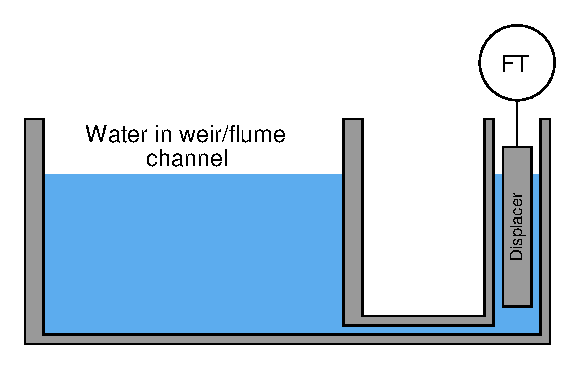
\includegraphics[width=15.5cm]{i00624x01.eps}$$

Nivåinstrumentet gir normalt karakteriseringen som lineariserer den ikke-lineære sammenhengen mellom flow og høyde. For ultralyd kan dette gjøres i samme digitale enhet som beregner nivå via ekkotid.

Det finnes også en lavteknologisk løsning. Hvis vi bruker displacer i stedet for digital ultralyd, kan vi oppnå samme karakterisering ved å velge riktig ikke-sylindrisk displacerform, slik at nivåhøyde i stillerøret ikke gir lineær oppdriftskraft i transmitteren.

\vskip 10pt

Anta transmitter på en Cippoletti-overfall, der flow varierer med 1.5-potens av nivåhøyde ($Q \propto H^{1.5}$). Velg riktig displacerprofil for å linearisere til direkte avlesbart flowsignal:

$$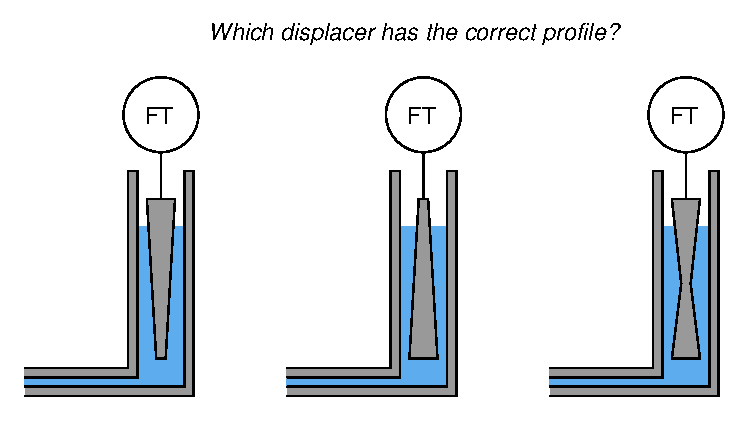
\includegraphics[width=15.5cm]{i00624x02.eps}$$

\underbar{file i00624}
%(END_QUESTION)





%(BEGIN_ANSWER)

$$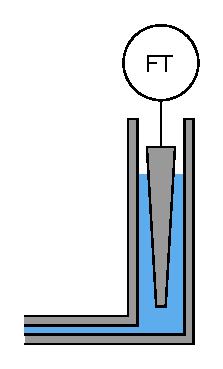
\includegraphics[width=15.5cm]{i00624x03.eps}$$

Forklar nå {\it hvorfor} displaceren må ha denne formen, og ikke de andre. Hint: skisser overfallets flow/høyde-overføringsfunksjon.

%(END_ANSWER)





%(BEGIN_NOTES)


%INDEX% Måling, flow: overføringsfunksjoner for overfall og renner

%(END_NOTES)

